\subsection{All-sky Imager}

The All-sky imager consist of a fisheye lens, an optical filter and a photon counter.

\begin{wrapfigure}{r}{0.5\textwidth} 
\vspace{-20pt}
  \begin{center}
    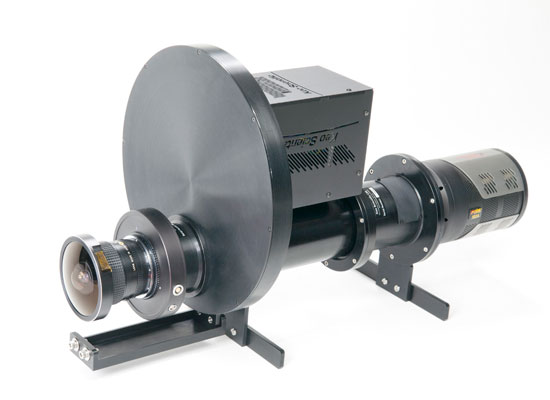
\includegraphics[width=0.4\textwidth]{Figures/Allsky/ERD_072.jpg}
    \caption{Allsky camera, Keo Scientific \fixme{add citation}}
    \label{fig:ACE}
  \end{center}
  \vspace{-20pt}
  \vspace{1pt}
\end{wrapfigure}


The fisheye lens gives a 180$^{\circ}$ view, so that th entire sky is covered. The optical filter gives us a image of only the wavelengths that is wanted, so that the only source is the Aurora. And the photon counter gives the intensity of the aurora in the part of the sky that equals the pixel size. When there is daylight or the full moon is visible may the aurora be to week for the all-sky imager, so the data cuts. 

The keograms are from the Ny \r{A}lesund allsky imager as the Longyearbyen imager didn't provide any data. 